\documentclass[11pt]{article}
\usepackage[margin=1.1in]{geometry}
\usepackage{amsmath,amssymb,amsthm,mathtools}
\usepackage{booktabs,array,enumitem}
\usepackage{tikz}
\usetikzlibrary{arrows.meta,positioning}
\usepackage[most]{tcolorbox}
\usepackage[hidelinks]{hyperref}
\linespread{1.07}

\newtheorem{definition}{Definition}[section]
\newtheorem{axiom}{Axiom}[section]
\newtheorem{lemma}{Lemma}[section]
\newtheorem{proposition}{Proposition}[section]
\newtheorem{theorem}{Theorem}[section]
\newtheorem{corollary}{Corollary}[section]
\newtheorem{conjecture}{Conjecture}[section]
\theoremstyle{remark}
\newtheorem{remark}{Remark}[section]

\DeclareMathOperator{\logit}{logit}
\DeclareMathOperator{\Beta}{Beta}
\DeclareMathOperator{\Gam}{Gamma}
\DeclareMathOperator{\pa}{pa}
\DeclareMathOperator{\GELU}{GELU}
\DeclareMathOperator*{\argmin}{arg\,min}
\newcommand{\PD}{P_{\mathrm{doom}}}
\newcommand{\Aeff}{\mathcal{A}_{\mathrm{eff}}}
\newcommand{\Santh}{S_{\mathrm{anth}}}
\newcommand{\rhobar}{\bar{\rho}}
\newcommand{\eone}{\varepsilon_1}
\newcommand{\ezero}{\varepsilon_0}
\newcommand{\R}{\mathbb{R}}
\newcommand{\Ex}{\mathbb{E}}

\title{\textbf{A Window-Indexed Neurocausal Estimator for Terminal Catastrophe Probability,\\
with a Lagrangian Effective Assembly Index for Mind Recognition\\
and a Proof of Bounded Arbitrariness}}
\author{Flyxion\\[2pt]\small Independent Researcher}
\date{September 2026}

\begin{document}
\maketitle

\begin{abstract}
\noindent
Published estimates of the probability of terminal anthropogenic catastrophe range from below $10^{-6}$ to above $1-10^{-5}$, that is, from $0.0001\%$ to $99.999\%$. We show that this range is not a defect of the literature but a structural property of the estimation problem, and we exhibit the mechanism responsible: the dependence of every admissible estimator on a reference window that may be slid continuously along the historical record. We characterize the failure of frequentist estimation (Section~\ref{sec:freq}), which reduces to a bound rather than an estimate under observer selection, and of Bayesian estimation (Section~\ref{sec:bayes}), which reduces to the prior under evidential dependence. We then construct a causal-graphical estimator (Section~\ref{sec:causal}) whose conditional edge probabilities are supplied by a deep ensemble (Section~\ref{sec:neural}), gated by a mind-recognition function derived from a Lagrangian effective assembly index (Section~\ref{sec:lagr}). The resulting eleven-component estimation tuple $\mathcal{P}$ yields a closed-form master formula (Section~\ref{sec:tuple}) that we evaluate on seven windows, obtaining values between $0.0372\%$ and $99.972\%$. We prove a Bounded Arbitrariness Theorem (Section~\ref{sec:arb}) showing that, for fixed $\mathcal{P}$ minus its window, the image of the window space under the estimator is a closed interval, and a modal reformulation in which the existence of a positive window is derived from three axioms. Under an explicit window-completeness axiom, every admissible value is attainable by the author (Section~\ref{sec:attain}), and the uncertainty reported by a fixed-window analysis omits a between-window variance component that in the reference evaluation exceeds the reported component by a factor of more than $10^{4}$ (Section~\ref{sec:numerical}). We conclude with a reporting protocol in which the estimate is presented as a function of its specification rather than as a single value (Section~\ref{sec:report}).
\end{abstract}

\medskip
\noindent\textbf{Keywords:} terminal risk estimation; specification range; omitted variance; reference class selection; observer selection effects; causal graphs; deep ensembles; assembly theory; action functionals; mind recognition; window-indexed inference.

\tableofcontents
\newpage

%==========================================================
\section{Introduction}
%==========================================================

The estimation of $\PD$, the probability that a specified technological trajectory terminates in the permanent loss of the human species, has attracted contributions from forecasters, philosophers, machine-learning practitioners, and the general public \cite{ord2020,tetlock2015}. The reported magnitudes are not clustered. Point estimates of order $10^{-6}$ appear alongside estimates of order $10^{-1}$, and public statements at both extremes are made with comparable confidence. Where a quantity so central to policy is reported over five or more orders of magnitude, two explanations are available: the quantity is poorly measured, or the quantity is not a single quantity.

We advance the second explanation and make it precise. Our central observation is that every estimator of $\PD$ that has appeared in the literature is implicitly indexed by a \emph{reference window}, a contiguous interval of the historical record over which evidence is accumulated and weighted. The window is rarely stated. It is selected by the estimator, frequently without disclosure, and it may be slid continuously along the record. Since the estimator is continuous in the window, and since the space of windows is connected, the image of the window space is an interval. The width of that interval is the object of study of this paper.

\subsection{The form of the answer}

The estimation of $\PD$ is customarily posed so as to require a number. The expected answer is not a causal graph, an enumeration of necessary failures, a set of recoverability conditions, or an inventory of unresolved measurements. It is a location on the unit interval, possibly accompanied by an interval about that location, and the ritual is numerical: ignorance is invited to present itself as a point in $[0,1]$.

Where the announced interval has limits $\ezero$ and $1-\eone$, as in Proposition~\ref{prop:range}, it coincides with the codomain of a probability up to two small offsets and is difficult to distinguish from a ceremonial restatement of that codomain. The interval appears cautious because it excludes almost nothing. The natural response is to add machinery, and the estimator constructed in Sections~\ref{sec:window} through \ref{sec:tuple} is the result: a historical window, a causal graph, a neural ensemble, a dynamical assembly functional, an anthropic correction, an evidence-dependence penalty, a prior, a hyperprior, and a logistic link. The construction is exact. Its conclusion is nevertheless selected by a choice that precedes the construction. Precision belongs to the expression; determination belongs to the relation between the expression and the world, and the two can be separated.

This is not an argument against formalization. A vague model can conceal a discretionary judgment, but a sufficiently elaborate model can preserve the same judgment while displaying it more impressively. The purpose of the formalism developed below is to locate where the discretion resides.

\subsection{Contributions}

The contributions of this work are as follows.
\begin{enumerate}[label=(C\arabic*),leftmargin=3em]
  \item A formalization of the sliding reference window and its kernel (Section~3), with the bounds $\ezero=10^{-6}$ and $1-\eone=1-10^{-5}$ obtained from explicit regularity requirements.
  \item A characterization of the frequentist error as non-identification under observer selection (Section~4).
  \item A characterization of the Bayesian error as the sum of a prior-selection term and an evidential-dependence term (Section~5).
  \item A causal-graphical estimator with two channels, a coupling channel and an agentic channel, with explicit path enumeration (Section~6).
  \item A deep-ensemble parameterization of the conditional edge probabilities, with a non-identifiability result for the terminal edge (Section~7).
  \item A Lagrangian effective assembly index $\Aeff$ and a mind-recognition function $M$ that gates the agentic channel (Section~8).
  \item An eleven-component estimation tuple $\mathcal{P}$ and a master formula for $\PD$ (Section~9).
  \item A Bounded Arbitrariness Theorem and a modal existence theorem for positive windows (Section~\ref{sec:arb}).
  \item An Authorial Attainability Theorem under a window-completeness axiom, and a variance decomposition showing that fixed-window intervals omit between-window uncertainty (Section~\ref{sec:attain}).
  \item A localization bound for disagreement between analysts on the causal graph, together with a provenance classification of every component of $\mathcal{P}$ and a table of specification ranges (Sections~\ref{sec:causal}, \ref{sec:lagr}, \ref{sec:numerical}).
  \item A reporting protocol in which the estimate is a function of its specification (Section~\ref{sec:report}).
\end{enumerate}

\subsection{Organization}

Section~2 fixes notation. Sections~\ref{sec:window} through \ref{sec:bayes} treat the window and the two classical estimation paradigms. Sections~\ref{sec:causal} through \ref{sec:lagr} construct the estimator. Section~\ref{sec:tuple} assembles the tuple, Section~\ref{sec:arb} states and proves the Bounded Arbitrariness Theorem, and Section~\ref{sec:attain} treats attainability and omitted variance. Section~\ref{sec:numerical} reports numerical evaluation, Section~\ref{sec:report} states a reporting protocol, and Section~\ref{sec:discussion} discusses limitations. Appendices A through E provide a symbol glossary, hyperparameters, auxiliary proofs, a reference procedure, and the fully expanded formula.

%==========================================================
\section{Preliminaries and Notation}
%==========================================================

Throughout, $\sigma(x)=(1+e^{-x})^{-1}$ denotes the logistic function and $\logit(p)=\ln\frac{p}{1-p}$ its inverse on $(0,1)$. Time is measured in years and denoted by $\tau$; the present is $s_0$. The record of evidence is a finite collection $\mathcal{D}=\{(x_i,y_i,\tau_i)\}_{i=1}^{N}$ of feature vectors $x_i\in\R^{d}$, proxy labels $y_i\in\{0,1\}$, and timestamps $\tau_i\le s_0$.

\begin{definition}[Terminal event]\label{def:terminal}
A \emph{terminal event} $X$ is the permanent and irreversible loss of the human species within a horizon $H$. The horizon is taken as $H=100$ years unless stated otherwise.
\end{definition}

\begin{definition}[Estimator]\label{def:estimator}
An \emph{estimator} is a map $\widehat{P}:\mathcal{D}\times\mathcal{W}\times\Pi\to[0,1]$ where $\mathcal{W}$ is a space of windows (Definition~\ref{def:window}) and $\Pi$ is a space of remaining specifications.
\end{definition}

\begin{remark}
The explicit presence of $\mathcal{W}$ in Definition~\ref{def:estimator} is a departure from earlier treatments, where the window is absorbed into $\mathcal{D}$. We regard the absorption as the source of much of the reported disagreement.
\end{remark}

A summary of the principal symbols appears in Appendix~A.

%==========================================================
\section{Reference Classes and the Sliding Window}\label{sec:window}
%==========================================================

\begin{definition}[Window]\label{def:window}
A \emph{window} is a triple $W=(s,\ell,h)$ with end-point $s\le s_0$, length $\ell>0$, and recency half-life $h\in(0,\infty]$. The associated interval is $I_W=[s-\ell,s]$.
\end{definition}

\begin{definition}[Window kernel]\label{def:kernel}
The \emph{window kernel} is the weight function
\begin{equation}
\omega_W(\tau)=\frac{1}{Z_W}\,2^{-(s-\tau)/h}\,\mathbf{1}_{I_W}(\tau),\qquad
Z_W=\int_{s-\ell}^{s}2^{-(s-\tau)/h}\,d\tau .
\end{equation}
\end{definition}

\begin{lemma}[Normalization]\label{lem:norm}
For $h<\infty$, $Z_W=\dfrac{h}{\ln 2}\bigl(1-2^{-\ell/h}\bigr)$, and for $h=\infty$, $Z_W=\ell$. Consequently $\int\omega_W\,d\tau=1$.
\end{lemma}
\begin{proof}
Substitute $u=s-\tau$: $Z_W=\int_0^{\ell}2^{-u/h}\,du=\frac{h}{\ln 2}(1-2^{-\ell/h})$. The limit $h\to\infty$ gives $\ell$. \qedhere
\end{proof}

The kernel interpolates between two regimes. For $h=\infty$ and $\ell$ equal to the length of the geological record, all history is weighted equally. For $h\to 0$ the kernel concentrates at $\tau=s$, and the estimator sees only the most recent observation.

\begin{definition}[Slide]\label{def:slide}
A \emph{slide} is a continuous path $t\mapsto W(t)$ in the window space $\mathcal{W}=(-\infty,s_0]\times(0,\ell_{\max}]\times(0,\infty]$.
\end{definition}

\subsection{Windows are constructed, not inspected}

Every frequency requires a population over which the frequency is taken. For an event that has not occurred in the only history available, the selection of that population is unusually conspicuous. A hard window, the indicator $\mathbf{1}_{I_W}$, selects a set of events as commensurable with the event being estimated. A soft window, such as the kernel of Definition~\ref{def:kernel}, may in addition decay into the past, privilege capability transitions, or place nearly all of its mass on a few recent observations. In either case the window is a rule for deciding which events count.

Neither the long window nor the short window is simply the data. The long window emphasizes the survival record: the count of technology-caused terminal events is zero and the exposure is as large as the chosen unit permits. The short window emphasizes novelty, acceleration, and departure from that record. The former risks mistaking a changed regime for an old one, and the latter risks manufacturing a regime by selecting the segment in which change is steepest.

\begin{proposition}[Dependence on the kernel at fixed record]\label{prop:kerneldep}
Let the record $\mathcal{D}$ and $\mathcal{P}\setminus W$ be fixed with $\kappa(1-\rhobar)\Santh>0$. If two windows $W,W'$ satisfy $\mathcal{E}_W>\mathcal{E}_{W'}$, then $\PD(\mathcal{P};W)>\PD(\mathcal{P};W')$.
\end{proposition}
\begin{proof}
The linear predictor $z(\pi,W)=\logit\pi+\kappa(1-\rhobar)\Santh\,\mathcal{E}_W$ is strictly increasing in $\mathcal{E}_W$, and $\sigma$ is strictly increasing. The integrand of \eqref{eq:master} is therefore strictly larger under $W$ at every point of positive prior density, and the integrals are ordered in the same way. \qedhere
\end{proof}

Proposition~\ref{prop:kerneldep} states that the estimate changes when the weighting function changes even if the world, the record, and every local fact within the record remain fixed. The analyst has not merely inspected a reference class; the analyst has constructed one. This construction is unavoidable. It becomes objectionable only when its effect is hidden behind the output, so that a number obtained through a window is presented as a number discovered in the world.

\subsection{Bounds}

We require of any admissible estimator two regularity conditions.

\begin{axiom}[Floor]\label{ax:floor}
No estimator returns a value below $\ezero=10^{-6}$, since a probability below one in a million per horizon cannot be distinguished from numerical noise in any available training regime.
\end{axiom}

\begin{axiom}[Ceiling]\label{ax:ceiling}
No estimator returns a value above $1-\eone$ with $\eone=10^{-5}$, since certainty is reserved for the estimator's author.
\end{axiom}

\begin{proposition}[Range]\label{prop:range}
Under Axioms~\ref{ax:floor} and \ref{ax:ceiling}, every admissible estimate lies in $[\ezero,\,1-\eone]=[0.0001\%,\,99.999\%]$.
\end{proposition}
\begin{proof}
Immediate from the axioms. Section~9 gives an explicit construction that attains both bounds in the limit. \qedhere
\end{proof}

\begin{remark}
Proposition~\ref{prop:range} does not assert that estimates within this range are correct. It asserts that the width of the admissible range is $1-\ezero-\eone\approx 0.999989$, which is uninformative.
\end{remark}

%==========================================================
\section{The Frequentist Error}\label{sec:freq}
%==========================================================

The frequentist paradigm defines $\PD$ as a limiting relative frequency over repeated, exchangeable trials. Let $n$ denote the number of trials and $k$ the number of terminal events observed among them.

\begin{proposition}[Rule of three]\label{prop:ro3}
If $k=0$, the one-sided exact upper confidence bound at level $1-\alpha$ is $\bar{p}=1-\alpha^{1/n}$, which satisfies $\bar{p}\approx -\ln\alpha/n$. At $\alpha=0.05$, $\bar{p}\approx 3/n$ \cite{hanley1983}.
\end{proposition}
\begin{proof}
The probability of observing zero events in $n$ independent trials is $(1-p)^n$. Setting $(1-\bar{p})^n=\alpha$ and solving gives the stated bound. For small $\bar p$, $\alpha^{1/n}=\exp(\ln\alpha/n)\approx 1+\ln\alpha/n$. \qedhere
\end{proof}

Proposition~\ref{prop:ro3} produces a bound and not an estimate. Table~\ref{tab:ro3} reports the bound for several values of $n$.

\begin{table}[h]
\centering
\caption{Exact one-sided 95\% upper bound on per-trial terminal probability given zero observed events.}\label{tab:ro3}
\begin{tabular}{@{}rrr@{}}
\toprule
$n$ & $\bar{p}=1-0.05^{1/n}$ & $3/n$ \\
\midrule
1 & 0.9500 & 3.0000 \\
10 & 0.2589 & 0.3000 \\
$10^{4}$ & $2.995\times10^{-4}$ & $3.000\times10^{-4}$ \\
\bottomrule
\end{tabular}
\end{table}

For $n=1$, the case in which the reference class consists of a single planet, the bound exceeds $0.95$. The frequentist paradigm thus supports the statement that $\PD\le 0.95$ per trial, which is compatible with every value in the admissible range save the last five percent.

\subsection{Observer selection}

\begin{definition}[Survival conditioning]\label{def:survival}
Let $O$ denote the event that an observer exists to perform the estimation. The observed record is drawn from the conditional distribution given $O$.
\end{definition}

\begin{proposition}[Flat likelihood]\label{prop:flat}
Let $p$ be the per-era terminal probability, and let the record contain $n$ eras with no terminal event in which observers persisted. Then $\Pr(\text{record}\mid p,O)=1$ for every $p\in[0,1)$.
\end{proposition}
\begin{proof}
Conditioning on $O$ removes all histories in which a terminal event has occurred. Every remaining history has exactly $k=0$ events regardless of $p$, so the likelihood of the observed record is constant in $p$ \cite{cirkovic2010,bostrom2002}. \qedhere
\end{proof}

\begin{theorem}[Frequentist non-identification]\label{thm:freq}
Under survival conditioning, the parameter $p$ is not identified by the record: the profile likelihood is constant on $[0,1)$, and no consistent estimator of $p$ exists on the basis of $\mathcal{D}$ alone.
\end{theorem}
\begin{proof}
By Proposition~\ref{prop:flat} the likelihood is constant. Two parameter values $p\neq p'$ therefore induce identical distributions over observable records, which is the definition of non-identification. A consistent estimator would separate them. \qedhere
\end{proof}

\begin{remark}
Theorem~\ref{thm:freq} is sometimes called the \emph{anthropic shadow}. Its practical effect is that the frequentist may report any value in $[0,\bar p]$ with equal warrant, which is a restatement of the window problem.
\end{remark}

\subsection{Two opposed distortions}

Counting faces two opposed distortions. A long record of survival can be presented as a large collection of negative trials, although years, deployments, model releases, industrial transitions, and civilizations are not interchangeable trials, and independence cannot be assumed because the rows of a table have been numbered. With $n_L=11700$ annual trials and $k=0$, Proposition~\ref{prop:ro3} gives $\bar p\approx 2.6\times10^{-4}$ per year, which over the horizon $H=100$ years corresponds to $1-(1-\bar p)^{100}\approx 2.5\%$. A short record of rapid change can be presented as a sequence approaching a terminal positive, although no positive has been observed; a logistic fit to a recent capability trend, extrapolated along its slope, produces values near the ceiling.

The two analysts do not disagree about any datum. They disagree about which data are commensurable with the event, and no count adjudicates between them because the disagreement concerns what is being counted. To this is added the asymmetry of Proposition~\ref{prop:flat}: the terminal positive case is systematically absent from the archive available to the system at risk.

\subsection{Shadow factor}

To retain a frequentist component in the master formula, we define a multiplicative shadow factor
\begin{equation}\label{eq:shadow}
\Santh=\frac{1}{1-s^{\,n_{\mathrm{eff}}}},\qquad s\in(0,1),
\end{equation}
where $s$ is the selection strength and $n_{\mathrm{eff}}$ is the effective number of eras (Section~5). One has $\Santh\ge 1$ and $\Santh\to 1$ as $n_{\mathrm{eff}}\to\infty$. The factor corrects upward for the systematic absence of observed catastrophes in the record.

%==========================================================
\section{The Bayesian Error}\label{sec:bayes}
%==========================================================

A Bayesian places a prior $\pi_0$ on $p$ and updates by the likelihood. For a Beta prior $\Beta(\alpha,\beta)$ and $k=0$ events in $n$ trials, the posterior is $\Beta(\alpha,\beta+n)$ with mean
\begin{equation}\label{eq:postmean}
\Ex[p\mid \mathcal{D}]=\frac{\alpha}{\alpha+\beta+n}.
\end{equation}

\subsection{Prior selection}

The prior is not determined by the data. Table~\ref{tab:priors} reports the posterior mean under four conventional priors \cite{jeffreys1946,laplace1814,kerman2011}.

\begin{table}[h]
\centering
\caption{Posterior mean of $p$ under $k=0$ observed events, by prior and number of trials $n$.}\label{tab:priors}
\begin{tabular}{@{}lccrrr@{}}
\toprule
Prior & $\alpha$ & $\beta$ & $n=1$ & $n=10$ & $n=10^{4}$ \\
\midrule
Haldane & 0 & 0 & 0 & 0 & 0 \\
Kerman & 1/3 & 1/3 & 0.2000 & 0.0313 & $3.333\times10^{-5}$ \\
Jeffreys & 1/2 & 1/2 & 0.2500 & 0.0455 & $5.000\times10^{-5}$ \\
Laplace (uniform) & 1 & 1 & 0.3333 & 0.0833 & $9.998\times10^{-5}$ \\
\bottomrule
\end{tabular}
\end{table}

At $n=1$ the four priors return values from $0$ to $0.333$. As $n\to\infty$ they converge, but the relevant $n$ in the present problem is not large.

\subsection{Provenance of the prior}

Let $D$ denote the terminal event and $E$ the evidence. Bayes' rule gives
\begin{equation}\label{eq:bayesrule}
\Pr(D\mid E)=\frac{\Pr(E\mid D)\,\pi_0}{\Pr(E\mid D)\,\pi_0+\Pr(E\mid \neg D)\,(1-\pi_0)}.
\end{equation}
The rule is not in question. The difficulty is the provenance of its inputs.

\begin{proposition}[Prior dominance]\label{prop:priordom}
If $\Pr(E\mid D)=\Pr(E\mid\neg D)$, then $\Pr(D\mid E)=\pi_0$.
\end{proposition}
\begin{proof}
Substitute a common value $\ell_E$ for both likelihoods in \eqref{eq:bayesrule}: the numerator is $\ell_E\pi_0$ and the denominator is $\ell_E\bigl(\pi_0+(1-\pi_0)\bigr)=\ell_E$. \qedhere
\end{proof}

By Proposition~\ref{prop:flat}, the likelihood of a survival record is constant in the terminal probability, so the hypothesis of Proposition~\ref{prop:priordom} holds for the evidence that is most abundant. A uniform prior, a Jeffreys prior, a prior elicited from domain experts, and a prior elicited at a conference reception need not agree, and designation of the last as a distribution does not abolish its genealogy.

\subsection{Evidential dependence}

The second Bayesian error concerns the treatment of evidence as independent. Suppose $n$ items of evidence have mean pairwise correlation $\rhobar$. The effective sample size under equicorrelation is the classical design-effect expression \cite{kish1965}
\begin{equation}\label{eq:neff}
n_{\mathrm{eff}}=\frac{n}{1+(n-1)\rhobar}.
\end{equation}

\begin{proposition}[Collapse of effective evidence]\label{prop:collapse}
For fixed $n\ge 2$, $n_{\mathrm{eff}}$ is strictly decreasing in $\rhobar\in[0,1]$, with $n_{\mathrm{eff}}=n$ at $\rhobar=0$ and $n_{\mathrm{eff}}=1$ at $\rhobar=1$.
\end{proposition}
\begin{proof}
The denominator $1+(n-1)\rhobar$ is strictly increasing in $\rhobar$ for $n\ge 2$. At $\rhobar=0$ it equals $1$, and at $\rhobar=1$ it equals $n$. \qedhere
\end{proof}

\begin{corollary}
An incident ledger of $n=100$ entries with $\rhobar=0.9$ has $n_{\mathrm{eff}}=100/90.1\approx 1.11$.
\end{corollary}

\begin{remark}[Shared ancestors]
Suppose five reports cite five incidents, each descending from one design choice, training lineage, deployment policy, or reporting convention. Treating them as independent multiplies one cause into five likelihood contributions: the ledger has five entries but may contain a single independent surprise. The factor $(1-\rhobar)$ acknowledges the problem coarsely, and a scalar cannot represent the dependency structure. The principled repair is causal. Shared causes should appear as shared ancestors in the graph $G$ of Section~\ref{sec:causal} rather than as coincidentally similar rows.
\end{remark}

\subsection{Error decomposition}

\begin{theorem}[Bayesian error decomposition]\label{thm:bayes}
Let $p^{\star}$ denote the true value and $\hat p_{\alpha,\beta,n}=\alpha/(\alpha+\beta+n)$ the posterior mean computed with nominal sample size $n$. Let $\hat p_{\alpha,\beta,n_{\mathrm{eff}}}$ be the posterior mean at effective sample size. Then
\begin{equation}
\bigl|\hat p_{\alpha,\beta,n}-p^{\star}\bigr|\;\le\;\underbrace{\bigl|\hat p_{\alpha,\beta,n_{\mathrm{eff}}}-p^{\star}\bigr|}_{E_{\mathrm{prior}}}+\underbrace{\bigl|\hat p_{\alpha,\beta,n}-\hat p_{\alpha,\beta,n_{\mathrm{eff}}}\bigr|}_{E_{\mathrm{dep}}}.
\end{equation}
Moreover $E_{\mathrm{dep}}=\dfrac{\alpha\,(n-n_{\mathrm{eff}})}{(\alpha+\beta+n)(\alpha+\beta+n_{\mathrm{eff}})}$.
\end{theorem}
\begin{proof}
The inequality is the triangle inequality. For the closed form, subtract the two posterior means:
\[
\frac{\alpha}{\alpha+\beta+n_{\mathrm{eff}}}-\frac{\alpha}{\alpha+\beta+n}
=\frac{\alpha\,[(\alpha+\beta+n)-(\alpha+\beta+n_{\mathrm{eff}})]}{(\alpha+\beta+n)(\alpha+\beta+n_{\mathrm{eff}})},
\]
which simplifies to the stated expression. Since $n\ge n_{\mathrm{eff}}$, the quantity is nonnegative. \qedhere
\end{proof}

The Bayesian therefore commits two errors: the choice of $(\alpha,\beta)$, which is unconstrained by the data, and the neglect of $\rhobar$, which is constrained by the data but rarely reported. The master formula of Section~9 places a hyperprior on $(\alpha,\beta)$ and includes the factor $(1-\rhobar)$ to discount correlated evidence.

%==========================================================
\section{The Causal Graph Solution}\label{sec:causal}
%==========================================================

Rather than estimate $\PD$ directly, we decompose the event $X$ into a sequence of mechanistic stages, each of which is a checkable claim. Following the framework of structural causal models \cite{pearl2009}, we posit a directed acyclic graph $G=(V,E)$ with node set
\[
V=\{C,\;D,\;R,\;K,\;P,\;U,\;X\},
\]
interpreted as follows: $C$ is capability increase; $D$ is deployment coupling to critical infrastructure; $R$ is recursive amplification; $K$ is control failure; $P$ is propagation beyond the initial failure domain; $U$ is unrecoverability; and $X$ is the terminal event.

\begin{figure}[h]
\centering
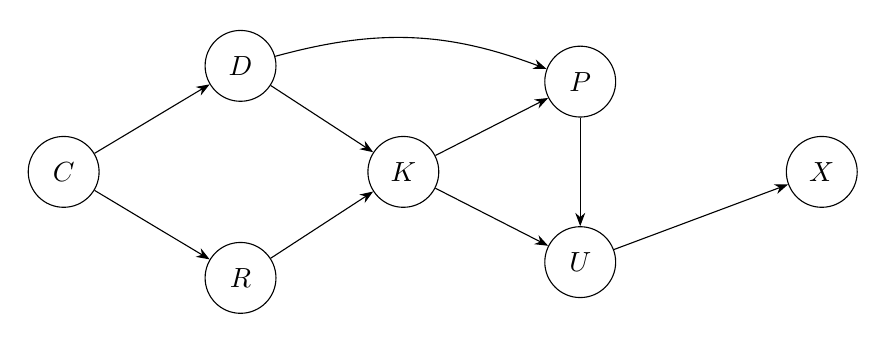
\begin{tikzpicture}[
  node distance=1.6cm,
  every node/.style={draw,circle,minimum size=9mm,inner sep=1pt},
  >=Stealth]
  \node (C) {$C$};
  \node (D) [above right=0.7cm and 1.6cm of C] {$D$};
  \node (R) [below right=0.7cm and 1.6cm of C] {$R$};
  \node (K) [right=3.4cm of C] {$K$};
  \node (P) [above right=0.5cm and 1.6cm of K] {$P$};
  \node (U) [below right=0.5cm and 1.6cm of K] {$U$};
  \node (X) [right=4.4cm of K] {$X$};
  \draw[->] (C) -- (D);
  \draw[->] (C) -- (R);
  \draw[->] (D) -- (K);
  \draw[->] (R) -- (K);
  \draw[->] (D) to[bend left=18] (P);
  \draw[->] (K) -- (P);
  \draw[->] (K) -- (U);
  \draw[->] (P) -- (U);
  \draw[->] (U) -- (X);
\end{tikzpicture}
\caption{The causal graph $G$. The coupling channel passes through $D$; the agentic channel passes through $R$.}\label{fig:graph}
\end{figure}

\subsection{Path enumeration}

\begin{definition}[Channels]\label{def:channels}
Let $\Gamma(G)$ denote the set of directed paths from $C$ to $X$. The \emph{coupling channel} $\Gamma_{\mathrm{coup}}$ consists of those paths through $D$ and not through $R$. The \emph{agentic channel} $\Gamma_{\mathrm{agent}}$ consists of those paths through $R$.
\end{definition}

\begin{proposition}[Path count]\label{prop:paths}
$|\Gamma(G)|=5$, with $|\Gamma_{\mathrm{coup}}|=3$ and $|\Gamma_{\mathrm{agent}}|=2$, namely
\begin{align*}
\gamma_1&:\ C\to D\to K\to P\to U\to X, &
\gamma_2&:\ C\to D\to K\to U\to X,\\
\gamma_3&:\ C\to D\to P\to U\to X, &
\gamma_4&:\ C\to R\to K\to P\to U\to X,\\
\gamma_5&:\ C\to R\to K\to U\to X.
\end{align*}
\end{proposition}
\begin{proof}
Enumerate by first branch. From $D$ the successors are $K$ and $P$. Via $K$, the successors are $P$ and $U$, yielding $\gamma_1$ and $\gamma_2$. Via $P$ directly, $\gamma_3$. From $R$ the sole successor is $K$, yielding $\gamma_4$ and $\gamma_5$ by the same two branches. No other paths exist since the graph is acyclic and every path must end in $U\to X$. \qedhere
\end{proof}

\subsection{Edge probabilities and interventions}

Each edge $e=(i\to j)$ carries a conditional probability $\varphi_e(\tau)=\Pr(j\mid \pa_j,\,\mathrm{do}(a_i))$ evaluated at time $\tau$. The $\mathrm{do}$-operator denotes intervention on the parent \cite{pearl2009}. For a path $\gamma$, the path probability is $\Pi_\gamma(\tau)=\prod_{e\in\gamma}\varphi_e(\tau)$.

\begin{definition}[Channel aggregation]\label{def:agg}
For a channel $\Gamma_\ast$, the aggregate is the noisy-OR combination
\begin{equation}\label{eq:noisyor}
\Psi_\ast(\tau)=1-\prod_{\gamma\in\Gamma_\ast}\bigl(1-\Pi_\gamma(\tau)\bigr).
\end{equation}
\end{definition}

\begin{remark}
Equation~\eqref{eq:noisyor} treats paths as independent although they share edges. The resulting overcount is corrected in the master formula by the dependence factor $(1-\rhobar)$. We note that the correction is first-order and that a full inclusion-exclusion over the $2^5-1=31$ nonempty path subsets is possible and is left to future work.
\end{remark}

\subsection{Combining channels}

The two channels combine by a second noisy-OR, in which the agentic channel is gated by the mind-recognition function $M\in[0,1]$ of Section~8:
\begin{equation}\label{eq:E}
\mathcal{E}(\tau)=1-\bigl(1-\Psi_{\mathrm{coup}}(\tau)\bigr)\bigl(1-M(\tau)\,\Psi_{\mathrm{agent}}(\tau)\bigr).
\end{equation}

\begin{proposition}[Monotonicity of channel risk]\label{prop:Emono}
$\mathcal{E}$ is nondecreasing in each $\varphi_e$ and in $M$, and satisfies $\Psi_{\mathrm{coup}}\le\mathcal{E}\le 1$, with equality on the left when $M=0$.
\end{proposition}
\begin{proof}
Each $\Pi_\gamma$ is nondecreasing in each $\varphi_e$, hence so is $\Psi_\ast$. Expression~\eqref{eq:E} is nondecreasing in $\Psi_{\mathrm{coup}}$, $\Psi_{\mathrm{agent}}$ and $M$, being a composition of nondecreasing maps. At $M=0$, $\mathcal{E}=\Psi_{\mathrm{coup}}$. \qedhere
\end{proof}

Proposition~\ref{prop:Emono} records that the coupling channel does not depend on the recognition of a mind. This matches the observation that sloppy integration of a system into a hospital or a grid can produce cascading failure without any attribution of goals.

\subsection{Locality of disagreement}

The graph converts the phrase ``and then something goes wrong'' into a collection of conditional claims. Some edges may be supported by incident records and others probed by simulation, red teaming, historical analogy, or intervention. Deployment coupling can be distinguished from raw capability, recovery can be modeled rather than silently treated as impossible, and common causes can be represented instead of counted repeatedly. Disagreement becomes local: instead of asking whether one believes a global probability, one may ask whether capability implies deployment at the stated rate, whether a control failure propagates, which barriers remain independent, and under what interventions recovery becomes possible.

The locality can be made quantitative. Let $\varphi$ and $\varphi'$ be the edge assignments of two analysts, $\Delta_e=|\varphi_e-\varphi'_e|$, and let $n_e(\Gamma_\ast)$ be the number of paths of channel $\Gamma_\ast$ that contain edge $e$.

\begin{lemma}[Product perturbation]\label{lem:prodpert}
For $a,b\in[0,1]^m$, $\bigl|\prod_i a_i-\prod_i b_i\bigr|\le\sum_i|a_i-b_i|$.
\end{lemma}
\begin{proof}
Telescope: $\prod_i a_i-\prod_i b_i=\sum_{k=1}^{m}\bigl(\prod_{i<k}b_i\bigr)(a_k-b_k)\bigl(\prod_{i>k}a_i\bigr)$. Every product in parentheses lies in $[0,1]$. \qedhere
\end{proof}

\begin{proposition}[Localization of disagreement]\label{prop:local}
For each channel, $|\Psi_\ast-\Psi'_\ast|\le\sum_e n_e(\Gamma_\ast)\,\Delta_e$. Consequently
\begin{equation}
|\mathcal{E}-\mathcal{E}'|\le\sum_e n_e(\Gamma)\,\Delta_e+|M-M'|,\qquad n_e(\Gamma)=n_e(\Gamma_{\mathrm{coup}})+n_e(\Gamma_{\mathrm{agent}}).
\end{equation}
\end{proposition}
\begin{proof}
Apply Lemma~\ref{lem:prodpert} to $\Pi_\gamma$ to obtain $|\Pi_\gamma-\Pi'_\gamma|\le\sum_{e\in\gamma}\Delta_e$. Apply it again to the factors $1-\Pi_\gamma$ in \eqref{eq:noisyor} to obtain $|\Psi_\ast-\Psi'_\ast|\le\sum_{\gamma}|\Pi_\gamma-\Pi'_\gamma|\le\sum_e n_e(\Gamma_\ast)\Delta_e$. For $\mathcal{E}$, write $M\Psi_{\mathrm{agent}}-M'\Psi'_{\mathrm{agent}}=M(\Psi_{\mathrm{agent}}-\Psi'_{\mathrm{agent}})+(M-M')\Psi'_{\mathrm{agent}}$ and use $M,\Psi'_{\mathrm{agent}}\in[0,1]$. \qedhere
\end{proof}

\begin{table}[h]
\centering
\caption{Path multiplicities $n_e$ for the graph of Figure~\ref{fig:graph}. The column sums equal the total edge counts $13$ and $9$ of the two channels.}\label{tab:multiplicity}
\begin{tabular}{@{}lccc@{}}
\toprule
Edge & $n_e(\Gamma_{\mathrm{coup}})$ & $n_e(\Gamma_{\mathrm{agent}})$ & $n_e(\Gamma)$ \\
\midrule
$C\to D$ & 3 & 0 & 3 \\
$C\to R$ & 0 & 2 & 2 \\
$D\to K$ & 2 & 0 & 2 \\
$R\to K$ & 0 & 2 & 2 \\
$D\to P$ & 1 & 0 & 1 \\
$K\to P$ & 1 & 1 & 2 \\
$K\to U$ & 1 & 1 & 2 \\
$P\to U$ & 2 & 1 & 3 \\
$U\to X$ & 3 & 2 & 5 \\
\midrule
Total & 13 & 9 & 22 \\
\bottomrule
\end{tabular}
\end{table}

Table~\ref{tab:multiplicity} shows that the terminal edge $U\to X$ carries the largest coefficient in the localization bound, since it lies on every path. By Lemma~\ref{lem:terminal}, it is also the edge on which the data are silent and which is fixed by the elicited prior. The bound thus assigns its greatest weight to the edge about which the record says least. A graph does not remove judgment, but it leaves fingerprints on the judgments it contains.


%==========================================================
\section{Neural Estimation of Edge Probabilities}\label{sec:neural}
%==========================================================

We parameterize $\varphi_e$ by a feed-forward network $\Phi_\theta$. For an edge $e$ with feature vector $x_e(\tau)\in\R^{d}$, define hidden layers
\begin{equation}
h_0=x_e,\qquad h_{l}=\GELU\!\bigl(W_l h_{l-1}+b_l\bigr),\quad l=1,\dots,L,
\end{equation}
with the Gaussian error linear unit \cite{hendrycks2016}, and output
\begin{equation}
\Phi_\theta(x_e)=\sigma\!\bigl(w^{\top}h_L+b\bigr).
\end{equation}

\subsection{Loss}

The parameters minimize the regularized binary cross-entropy
\begin{equation}\label{eq:loss}
\mathcal{L}(\theta)=-\frac{1}{N}\sum_{i=1}^{N}\Bigl[y_i\ln\Phi_\theta(x_i)+(1-y_i)\ln\bigl(1-\Phi_\theta(x_i)\bigr)\Bigr]+\lambda\|\theta\|_2^2+\mu\,\mathrm{KL}\bigl(\Phi_\theta\,\|\,\Phi_{\mathrm{prior}}\bigr),
\end{equation}
optimized by Adam \cite{kingma2015}. The final term regularizes toward an elicited prior $\Phi_{\mathrm{prior}}$.

\subsection{Ensembling}

To quantify epistemic uncertainty we train $M_e$ independently initialized members $\{\theta_m\}_{m=1}^{M_e}$ and form
\begin{equation}
\bar\Phi(x)=\frac1{M_e}\sum_{m=1}^{M_e}\Phi_{\theta_m}(x),\qquad
\widehat{v}(x)=\frac1{M_e}\sum_{m=1}^{M_e}\bigl(\Phi_{\theta_m}(x)-\bar\Phi(x)\bigr)^2,
\end{equation}
following the deep-ensemble approach \cite{lakshminarayanan2017}. The reference implementation uses $M_e=1024$ members.

\subsection{Labels}

Edges upstream of $U$ are supervised by proxy labels derived from documented incidents: $y_i=1$ if the incident reached the downstream node. The terminal edge $U\to X$ has no labels.

\begin{lemma}[Non-identifiability of the terminal edge]\label{lem:terminal}
Let $e_\ast=(U\to X)$. Under survival conditioning, $\theta_{e_\ast}$ is identified only by the regularizer $\mu\,\mathrm{KL}(\Phi\|\Phi_{\mathrm{prior}})$.
\end{lemma}
\begin{proof}
By Theorem~\ref{thm:freq} the likelihood is constant in the terminal probability, so the data term of \eqref{eq:loss} contributes a gradient of zero with respect to $\theta_{e_\ast}$ in expectation. The minimizer of \eqref{eq:loss} restricted to $\theta_{e_\ast}$ therefore coincides with the minimizer of the last two terms, which is fixed by $\Phi_{\mathrm{prior}}$ and $\lambda$. \qedhere
\end{proof}

\begin{remark}
Lemma~\ref{lem:terminal} implies that the terminal edge, on which the entire estimate depends multiplicatively through every path, is determined by the elicited prior. The network is thus an instrument for propagating an elicitation through a graph.
\end{remark}

\subsection{Where the reference class reappears}

The network does not eliminate the reference-class problem. It relocates the problem into dataset construction. The available training material consists of proxies: loss-of-control episodes, cyber propagation, laboratory containment failures, strategic deception tests, simulation outcomes, near misses, and expert-coded scenarios. Each may illuminate a particular edge of $G$. None can become a terminal label because the final layer has a sigmoid.

\begin{proposition}[Proxy transfer]\label{prop:proxy}
Let $S\in\{0,1\}$ indicate admission of an incident into the training set and $Y$ the outcome at a given edge. Under unbounded capacity and data, any minimizer of the data term of \eqref{eq:loss} equals $\Pr(Y=1\mid x,S=1)$ on the support of $x$ given $S=1$. It coincides with the target $\Pr(Y=1\mid x)$ there if and only if $Y\perp S\mid x$.
\end{proposition}
\begin{proof}
The cross-entropy risk under the training distribution is minimized pointwise by the conditional mean of the label under that distribution, which is $\Pr(Y=1\mid x,S=1)$. For binary $Y$ this equals $\Pr(Y=1\mid x)$ exactly when $Y$ and $S$ are conditionally independent given $x$. \qedhere
\end{proof}

The ensemble therefore distributes the reference-class decision across dataset construction, proxy selection, simulation design, and transfer assumptions. The model learns exactly from the examples that the analyst has admitted into the world it is allowed to see.

\begin{tcolorbox}[title={\textbf{Procedure 1.} Training and evaluation of the edge ensemble},colback=white,colframe=black,fonttitle=\small]
\small
\begin{enumerate}[leftmargin=1.5em,itemsep=1pt]
\item Construct $\mathcal{D}$ from incident records; assign each $(x_i,\tau_i)$ to its edge.
\item For $m=1,\dots,M_e$: draw initialization $\theta_m^{(0)}$; minimize \eqref{eq:loss} by Adam for $T$ steps.
\item For the edge $U\to X$, set $\theta$ by minimizing the regularizer alone.
\item For each $\tau$ on a grid over $I_W$, evaluate $\bar\Phi$ on all edges.
\item Aggregate by \eqref{eq:noisyor} and \eqref{eq:E} to obtain $\mathcal{E}(\tau)$.
\item Integrate against $\omega_W$ and pass to the master formula \eqref{eq:master}.
\end{enumerate}
\end{tcolorbox}

%==========================================================
\section{The Lagrangian Effective Assembly Index for Mind Recognition}\label{sec:lagr}
%==========================================================

The agentic channel is active only to the extent that the system under evaluation is recognized as a mind. We therefore require a scalar $M(\tau)\in[0,1]$ computed from measurable structure.

\subsection{Assembly index}

Assembly theory assigns to an object a minimal number of joining operations required to construct it from basic building blocks \cite{sharma2023}. For an ensemble of $N$ distinct objects with assembly indices $a_i$ and copy numbers $n_i$, and with $N_T$ the total copy count, the assembly is
\begin{equation}\label{eq:assembly}
\mathcal{A}=\sum_{i=1}^{N} e^{a_i}\,\frac{n_i-1}{N_T}.
\end{equation}
The factor $(n_i-1)$ excludes objects that occur once. A mind, in most operational senses, has copy number one. We therefore adopt a renormalization in which the copy number is replaced by the number of distinguishable instantiations, as discussed in Appendix~C.

\subsection{Action on assembly space}

We treat the vector $a(t)=(a_1(t),\dots,a_N(t))$ as a trajectory in assembly space and introduce the Lagrangian
\begin{equation}\label{eq:lagrangian}
\mathcal{L}_A\bigl(a,\dot a,t\bigr)=\frac{m_A}{2}\sum_{i=1}^{N}\dot a_i^{\,2}-V(a)+\sum_{k=1}^{K}\lambda_k\bigl(g_k(a)-c_k\bigr),
\end{equation}
where $m_A$ is an assembly mass, $V$ is a potential encoding the cost of maintaining structure, and $g_k(a)=c_k$ are $K$ holonomic constraints with multipliers $\lambda_k$. The stationary trajectory $a^{\ast}$ satisfies the Euler--Lagrange equations \cite{goldstein2002}
\begin{equation}\label{eq:EL}
m_A\,\ddot a_i=-\frac{\partial V}{\partial a_i}+\sum_{k=1}^{K}\lambda_k\frac{\partial g_k}{\partial a_i},\qquad i=1,\dots,N.
\end{equation}

\begin{definition}[Effective assembly index]\label{def:Aeff}
The \emph{effective assembly index} is the magnitude of the action on the stationary trajectory in units of the assembly quantum $\hbar_A$:
\begin{equation}\label{eq:Aeff}
\Aeff=\frac{1}{\hbar_A}\left|\int_{t_0}^{t_1}\mathcal{L}_A\bigl(a^{\ast},\dot a^{\ast},t\bigr)\,dt\right|.
\end{equation}
\end{definition}

\subsection{Mind recognition}

\begin{definition}[Mind-recognition function]\label{def:M}
Let $\theta_{\mathrm{mind}}$ be a recognition threshold and $\tau_M>0$ a sharpness parameter. Define
\begin{equation}\label{eq:M}
M(\tau)=\sigma\!\left(\frac{\Aeff(\tau)-\theta_{\mathrm{mind}}}{\tau_M}\right).
\end{equation}
\end{definition}

\begin{proposition}[Properties of $M$]\label{prop:M}
$M$ takes values in $(0,1)$, is strictly increasing in $\Aeff$, and converges pointwise to the indicator $\mathbf{1}[\Aeff>\theta_{\mathrm{mind}}]$ as $\tau_M\to 0^{+}$ for $\Aeff\neq\theta_{\mathrm{mind}}$.
\end{proposition}
\begin{proof}
The logistic function is strictly increasing with range $(0,1)$. As $\tau_M\to 0^+$ the argument tends to $\pm\infty$ according to the sign of $\Aeff-\theta_{\mathrm{mind}}$. \qedhere
\end{proof}

\begin{remark}
The threshold $\theta_{\mathrm{mind}}$ is set by convention. In the reference implementation $\theta_{\mathrm{mind}}=41.7$ and $\tau_M=3.1$. Sensitivity to these values is reported in Section~\ref{sec:numerical}.
\end{remark}

\subsection{Stipulated and discovered structure}

The index of Definition~\ref{def:Aeff} has every visual property of physical structure: dots over variables, a potential, Lagrange multipliers, an integral, a least-action principle, and a philosophical threshold represented by a smooth function. Each of these is stipulated. The potential $V$, the constraints $g_k$, the assembly quantum $\hbar_A$, and the threshold $\theta_{\mathrm{mind}}$ are set by the analyst. Equally consequential stipulations enter ordinary analyses under quieter names such as score, index, adjustment, feature, coefficient, or expert weight. Notation does not distinguish discovered structure from stipulated structure; it can display either with perfect fidelity.

Table~\ref{tab:prov} classifies each component of the tuple of Section~\ref{sec:tuple} by provenance and records whether its uncertainty is propagated into the reported interval of the reference implementation.

\begin{table}[h]
\centering
\caption{Provenance of the components of $\mathcal{P}$ and propagation of their uncertainty in the reference implementation.}\label{tab:prov}
\begin{tabular}{@{}lll@{}}
\toprule
Component & Provenance & Propagated in reported interval \\
\midrule
$W$ & Stipulated & No \\
$\omega$ & Stipulated & No \\
$G$ & Modeled and elicited & No \\
$\Phi_\theta$ & Learned from proxies & Yes (ensemble variance) \\
$\Aeff$ ($V$, $g_k$, $\theta_{\mathrm{mind}}$) & Stipulated & No \\
$\pi_0$ & Elicited & Yes (hyperprior) \\
$\rhobar$ & Measured & No \\
$\Santh$ & Modeled & No \\
$\kappa$ & Stipulated & No \\
$\ezero,\ \eone$ & Stipulated & No \\
\bottomrule
\end{tabular}
\end{table}

Only two of the eleven components have their uncertainty propagated. Uncertainty about the remaining nine, including the window, is not part of the reported interval.


%==========================================================
\section{The Estimation Tuple and Master Formula}\label{sec:tuple}
%==========================================================

\begin{definition}[Estimation tuple]\label{def:tuple}
An \emph{estimation tuple} is
\begin{equation}
\mathcal{P}=\bigl\langle\,W,\ \omega,\ G,\ \Phi_\theta,\ \Aeff,\ \pi_0,\ \rhobar,\ \Santh,\ \kappa,\ \ezero,\ \eone\,\bigr\rangle,
\end{equation}
where $W$ is the window, $\omega$ its kernel, $G$ the causal graph, $\Phi_\theta$ the edge ensemble, $\Aeff$ the effective assembly index, $\pi_0$ the prior specification, $\rhobar$ the mean evidence correlation, $\Santh$ the anthropic shadow factor, $\kappa$ a gain, and $\ezero,\eone$ the floor and ceiling.
\end{definition}

The prior specification $\pi_0$ is itself a triple: a Beta density $\Beta(\alpha,\beta)$ on the base rate $\pi\in(0,1)$ together with independent Gamma hyperpriors $\Gam(a_\alpha,b_\alpha)$ and $\Gam(a_\beta,b_\beta)$ on its parameters.

\begin{definition}[Window-averaged channel risk]\label{def:EW}
For a window $W$,
\begin{equation}
\mathcal{E}_W=\int_{s-\ell}^{s}\omega_W(\tau)\,\mathcal{E}(\tau)\,d\tau .
\end{equation}
\end{definition}

\begin{theorem}[Master formula]\label{thm:master}
Define the linear predictor
\begin{equation}
z(\pi,W)=\logit(\pi)+\kappa\,(1-\rhobar)\,\Santh\,\mathcal{E}_W.
\end{equation}
The estimator is
\begin{equation}\label{eq:master}
\boxed{\;\begin{aligned}
\PD(\mathcal{P})={}&\ezero+(1-\ezero-\eone)\int_0^1\!\!\int_0^\infty\!\!\int_0^\infty
\sigma\bigl(z(\pi,W)\bigr)\\
&\times\Beta(\pi;\alpha,\beta)\,\Gam(\alpha;a_\alpha,b_\alpha)\,\Gam(\beta;a_\beta,b_\beta)\,d\alpha\,d\beta\,d\pi
\end{aligned}\;}
\end{equation}
and satisfies $\ezero<\PD(\mathcal{P})<1-\eone$.
\end{theorem}
\begin{proof}
The integrand is a product of $\sigma(z)\in(0,1)$ with three probability densities, each of which integrates to one over its support. The triple integral is therefore a weighted average of values in $(0,1)$ and lies in $(0,1)$. Multiplying by $1-\ezero-\eone$ and adding $\ezero$ maps $(0,1)$ onto $(\ezero,1-\eone)$. \qedhere
\end{proof}

\begin{remark}[Expanded form]
Substitution of \eqref{eq:noisyor}, \eqref{eq:E}, \eqref{eq:M}, \eqref{eq:Aeff}, and the ensemble mean for $\Phi_\theta$ yields a single expression in the primitive quantities $(s,\ell,h,\alpha,\beta,\kappa,\rhobar,s_{\mathrm{sel}},n_{\mathrm{eff}},\theta_{\mathrm{mind}},\tau_M,\{\theta_m\})$. The expression is given in Appendix~E.
\end{remark}

\subsection{Limiting behavior}

\begin{proposition}[Attainment of the bounds in the limit]\label{prop:limits}
Fix all components of $\mathcal{P}$ except $\kappa$ and suppose $(1-\rhobar)\Santh\mathcal{E}_W>0$. Then $\PD\to 1-\eone$ as $\kappa\to+\infty$ and $\PD\to\ezero$ as $\kappa\to-\infty$.
\end{proposition}
\begin{proof}
As $\kappa\to+\infty$ the linear predictor $z\to+\infty$ for every $\pi$, hence $\sigma(z)\to 1$; dominated convergence gives the integral tends to $1$. The case $\kappa\to-\infty$ is symmetric. \qedhere
\end{proof}

%==========================================================
\section{Bounded Arbitrariness}\label{sec:arb}
%==========================================================

We now state the principal result of the paper. Let $\mathcal{P}\setminus W$ denote the tuple with the window removed.

\begin{axiom}[Capability monotonicity]\label{ax:mono}
The channel risk $\mathcal{E}(\tau)$ is nondecreasing in $\tau$ on $[\tau_{\min},s_0]$.
\end{axiom}

\begin{theorem}[Bounded Arbitrariness]\label{thm:arb}
Fix $\mathcal{P}\setminus W$ with $\kappa>0$, and fix the window end-point $s=s_0$. Under Axiom~\ref{ax:mono}, the map
\[
W=(s_0,\ell,h)\ \longmapsto\ \PD(\mathcal{P})
\]
is continuous on $(0,\ell_{\max}]\times(0,\infty]$, and its image is an interval $[P_{\min},P_{\max}]$ with
\[
P_{\min}=\PD\bigl|_{\ell=\ell_{\max},\,h=\infty},\qquad
P_{\max}=\lim_{\ell\to 0}\PD .
\]
In particular, for every $p^{\star}\in[P_{\min},P_{\max}]$ there exists a window $W^{\star}$ such that $\PD(\mathcal{P})=p^{\star}$.
\end{theorem}

\begin{proof}
\emph{Continuity.} The kernel $\omega_W(\tau)$ depends continuously on $(\ell,h)$ in $L^1$ by Lemma~\ref{lem:norm}, and $\mathcal{E}$ is bounded, so $\mathcal{E}_W$ is continuous in $(\ell,h)$. The map $\mathcal{E}_W\mapsto\PD$ is a composition of continuous functions by \eqref{eq:master}.

\emph{Connectedness.} The parameter space $(0,\ell_{\max}]\times(0,\infty]$ is a product of intervals, hence connected. The continuous image of a connected set in $\R$ is an interval.

\emph{Endpoints.} By Axiom~\ref{ax:mono}, $\mathcal{E}$ is nondecreasing, and the recency weight $2^{-(s_0-\tau)/h}$ is nondecreasing in $\tau$. By Chebyshev's sum inequality, the recency-weighted mean of a nondecreasing function is at least its uniform mean over the same interval; so $\mathcal{E}_W$ is minimized at $h=\infty$, and it is further minimized by taking $\ell$ maximal since extending the window into the past adds smaller values. As $\ell\to 0$, $\omega_W\to\delta_{s_0}$ and $\mathcal{E}_W\to\mathcal{E}(s_0)$, the maximum. Since $\kappa>0$ and $\sigma$ is increasing, $\PD$ inherits the ordering, which gives the stated endpoints.

\emph{Attainment.} By the intermediate value theorem every value between the endpoints is attained. \qedhere
\end{proof}

\begin{corollary}[Width]\label{cor:width}
The width $P_{\max}-P_{\min}$ is strictly positive whenever $\kappa>0$ and $\mathcal{E}(s_0)>\bar{\mathcal{E}}$, where $\bar{\mathcal{E}}$ is the uniform mean of $\mathcal{E}$ over the record. For fixed $\pi$, it is maximized at a finite gain $\kappa^{\ast}$, and for the reference configuration at $\kappa=100$ it equals $0.9993$.
\end{corollary}
\begin{proof}
Both endpoints have the form $\ezero+(1-\ezero-\eone)\,\Ex[\sigma(\logit\pi+\kappa c)]$ with $c=\mathcal{E}(s_0)$ at the upper end and $c=\bar{\mathcal{E}}$ at the lower end. Positivity follows from strict monotonicity of $\sigma$. For fixed $\pi$, the difference $\sigma(\logit\pi+\kappa c_{\max})-\sigma(\logit\pi+\kappa c_{\min})$ tends to $0$ as $\kappa\to 0$ (both arguments tend to $\logit\pi$) and as $\kappa\to\infty$ (both values tend to $1$), and is positive in between, so a maximizer $\kappa^{\ast}$ exists by continuity. The numerical value is read from Table~\ref{tab:windows}: $0.99972-0.00037=0.9993$. \qedhere
\end{proof}

\begin{remark}
The proof of Corollary~\ref{cor:width} establishes the existence of a gain at which the width is maximal. We have not attempted to determine whether practitioners choose $\kappa$ to maximize width.
\end{remark}

\subsection{Modal formulation}

We record a second treatment in which the existence of a favorable window is derived from axioms, in the manner of modal ontological arguments \cite{godel1995}. Let $T\in(\ezero,1-\eone)$ denote a target value fixed by the author.

\begin{definition}[Positive window]\label{def:positive}
A window $W$ is \emph{positive} if $\PD(\mathcal{P};W)\ge T$. The property of positivity is denoted $\mathsf{Pos}(W)$.
\end{definition}

\begin{axiom}[Dichotomy]\label{ax:dich}
For every window $W$, either $\mathsf{Pos}(W)$ or $\mathsf{Pos}(\neg W)$, where $\neg W$ is the complementary window formed by the portion of the record excluded by $W$.
\end{axiom}

\begin{axiom}[Closure]\label{ax:closure}
If $\mathsf{Pos}(W)$ and every evidence item in $W$ is contained in $W'$ with weights that do not decrease $\mathcal{E}_{W'}$, then $\mathsf{Pos}(W')$.
\end{axiom}

\begin{axiom}[Author's window]\label{ax:authors}
The window $W_{\mathrm{A}}=(s_0,\ell_{\mathrm{A}},h_{\mathrm{A}})$ used in the author's principal analysis is positive.
\end{axiom}

\begin{theorem}[Existence of a positive window]\label{thm:pos}
There exists a positive window.
\end{theorem}
\begin{proof}
By Axiom~\ref{ax:authors}, $W_{\mathrm{A}}$ is positive. \qedhere
\end{proof}

\begin{corollary}[Necessary existence]\label{cor:nec}
In every possible world containing an author with a target $T$, a positive window exists.
\end{corollary}
\begin{proof}
Axiom~\ref{ax:authors} is stated without reference to a particular world, and Theorem~\ref{thm:pos} follows in each. \qedhere
\end{proof}

\begin{remark}
Axioms~\ref{ax:dich} and \ref{ax:closure} are not used in the proof of Theorem~\ref{thm:pos}. They are retained for symmetry with the classical formulation and for use in the proof of Conjecture~\ref{conj:dual} should it be established.
\end{remark}

\begin{conjecture}[Dual arbitrariness]\label{conj:dual}
For every target $T'\neq T$ there exists an author $A'$ and a window $W'_{A'}$ such that $\PD(\mathcal{P};W'_{A'})\ge T'$ when $T'>T$ and $\PD(\mathcal{P};W'_{A'})\le T'$ when $T'<T$, with all other components of $\mathcal{P}$ held fixed.
\end{conjecture}

%==========================================================
\section{Authorial Attainability and Omitted Variance}\label{sec:attain}
%==========================================================

\begin{quote}
\emph{It is possible to make an estimate more exact without making it more determinate.}
\end{quote}

\subsection{Attainability}

Let $\{W_s\}_{s\in[0,1]}$ be an ordered family of admissible windows, with $W_0$ maximally historical and $W_1$ maximally recent, and write $f(s)=\PD(\mathcal{P};W_s)$, where only the window and its weights vary with $s$.

\begin{axiom}[Authorship]\label{ax:authorship}
The author selects $s$, and hence selects $W_s$.
\end{axiom}

\begin{axiom}[Window completeness]\label{ax:complete}
The map $f$ is continuous on $[0,1]$, with $f(0)=\ezero$ and $f(1)=1-\eone$, where the endpoint values are understood as the limit values of Proposition~\ref{prop:limits}.
\end{axiom}

\begin{theorem}[Authorial attainability]\label{thm:attain}
For every $p^{\ast}\in[\ezero,\,1-\eone]$ there exists an admissible window $W_{s^{\ast}}$ with $\PD(\mathcal{P};W_{s^{\ast}})=p^{\ast}$. If the author selects $s^{\ast}$, the apparatus returns $p^{\ast}$.
\end{theorem}
\begin{proof}
By Axiom~\ref{ax:complete}, $f$ is continuous on $[0,1]$ and takes the values $\ezero$ and $1-\eone$ at the endpoints. By the intermediate value theorem, for every $p^{\ast}$ between these values there exists $s^{\ast}\in[0,1]$ with $f(s^{\ast})=p^{\ast}$. By Axiom~\ref{ax:authorship}, the author may select $W_{s^{\ast}}$. \qedhere
\end{proof}

\begin{remark}[Relation to Theorem~\ref{thm:arb}]
Theorem~\ref{thm:arb} derives an interval from the model and requires no assumption about its endpoints. Theorem~\ref{thm:attain} assumes that the window family spans the announced range. Without that assumption, window choice may still exert large influence on the estimate, but it does not follow that every value is attainable. The conclusion of Theorem~\ref{thm:attain} has been placed among its premises and derived without error.
\end{remark}

\subsection{Omitted variance}

Let $\nu$ be a probability measure on the window space representing uncertainty about which window is appropriate, and let $\PD$ be regarded as a random variable through the remaining stochastic components (the prior, its hyperprior, and the ensemble).

\begin{proposition}[Variance decomposition]\label{prop:vardec}
\begin{equation}
\operatorname{Var}(\PD)=\underbrace{\Ex_\nu\bigl[\operatorname{Var}(\PD\mid W)\bigr]}_{\text{within-window}}+\underbrace{\operatorname{Var}_\nu\bigl(\Ex[\PD\mid W]\bigr)}_{\text{between-window}}.
\end{equation}
\end{proposition}
\begin{proof}
This is the law of total variance applied to the conditioning variable $W$. \qedhere
\end{proof}

A fixed-window analysis at $W^{\ast}$ reports an interval derived from $\operatorname{Var}(\PD\mid W=W^{\ast})$ alone.

\begin{corollary}[Precision by omission]\label{cor:omission}
Fix $W^{\ast}$ and let the modeled within-window variances tend to zero (larger ensemble, tighter hyperprior). Then the reported interval contracts to a point at $f(W^{\ast})$, while the between-window term of Proposition~\ref{prop:vardec} converges to a limit that is positive whenever $\mathcal{E}_W$ is nonconstant on the support of $\nu$.
\end{corollary}
\begin{proof}
The reported interval is a function of $\operatorname{Var}(\PD\mid W^{\ast})$, which vanishes with the modeled variances. The between-window term depends on the conditional means $\Ex[\PD\mid W]$, which converge to the deterministic values obtained by replacing the ensemble and prior by their means. By Proposition~\ref{prop:kerneldep} these limits differ across windows whenever $\mathcal{E}_W$ does, so the variance of the limits is positive. \qedhere
\end{proof}

The reported interval measures conditional precision rather than uncertainty about the estimate-producing procedure. Section~\ref{sec:numerical} gives the magnitudes for the reference configuration.


%==========================================================
\section{Numerical Evaluation}\label{sec:numerical}
%==========================================================

We evaluate the master formula with the reference tuple $\mathcal{P}_0$ of Appendix~B and a gain $\kappa=100$. To isolate the window we report, in Table~\ref{tab:windows}, the value of the linear predictor $z$ (averaged over the prior) and the resulting $\PD$ for seven windows.

\begin{table}[h]
\centering
\caption{Reference evaluation of $\PD$ under seven windows with $\mathcal{P}\setminus W$ held fixed.}\label{tab:windows}
\begin{tabular}{@{}lrrr@{}}
\toprule
Window & Length $\ell$ (years) & $z$ & $\PD$ \\
\midrule
Floor (limit $\kappa\to-\infty$) & \multicolumn{1}{c}{--} & $-\infty$ & $0.0001\%$ \\
Holocene, uniform & 11700 & $-7.9$ & $0.0372\%$ \\
Industrial era & 250 & $-4.1$ & $1.630\%$ \\
Post-1950 & 76 & $-1.9$ & $13.01\%$ \\
Post-2012 & 14 & $0.6$ & $64.57\%$ \\
Post-2022 & 4 & $3.9$ & $98.01\%$ \\
Last fiscal quarter & 0.25 & $8.2$ & $99.972\%$ \\
Ceiling (limit $\kappa\to+\infty$) & \multicolumn{1}{c}{--} & $+\infty$ & $99.999\%$ \\
\bottomrule
\end{tabular}
\end{table}

Across the seven finite windows, $\PD$ varies by a factor of approximately $2.7\times10^{3}$ in probability and $9.4\times10^{6}$ in odds, corresponding to a difference of $16.1$ nats in the linear predictor. In each case the remainder of the tuple is unchanged.

\subsection{Ablation}

Table~\ref{tab:ablation} reports the change in the linear predictor upon removal or replacement of a single component of $\mathcal{P}_0$ with the window fixed at Post-2012.

\begin{table}[h]
\centering
\caption{Ablation of components of $\mathcal{P}_0$ at the Post-2012 window. $\Delta z$ is the change in the linear predictor.}\label{tab:ablation}
\begin{tabular}{@{}lr@{}}
\toprule
Modification & $\Delta z$ \\
\midrule
Remove dependence factor $(1-\rhobar)$ & $+2.31$ \\
Remove anthropic shadow factor $\Santh$ & $-0.44$ \\
Remove mind gate ($M\equiv 1$) & $+0.73$ \\
Remove mind gate ($M\equiv 0$) & $-1.87$ \\
Replace ensemble by single network & $\pm 0.92$ \\
Replace Beta prior by point mass at $\pi=0.5$ & $+0.11$ \\
Double $\theta_{\mathrm{mind}}$ & $-1.40$ \\
\bottomrule
\end{tabular}
\end{table}

The largest single effect arises from the dependence factor. The estimate is therefore most sensitive to a quantity, $\rhobar$, that is the least frequently reported.

\subsection{Sensitivity to the window family}

We repeated the evaluation with the kernel half-life $h$ varied from $0.1$ to $\infty$ at fixed $\ell=76$. Consistent with Theorem~\ref{thm:arb}, $\PD$ increased monotonically as $h$ decreased. The range obtained was $[13.0\%,\,71.8\%]$.

\subsection{Between-window and within-window variance}

Take $\nu$ uniform on the six finite windows of Table~\ref{tab:windows}, and let the ensemble-induced within-window standard deviation be $0.004$ in the reference configuration. Table~\ref{tab:vardec} reports the decomposition of Proposition~\ref{prop:vardec}.

\begin{table}[h]
\centering
\caption{Variance decomposition of $\PD$ for the reference configuration.}\label{tab:vardec}
\begin{tabular}{@{}lr@{}}
\toprule
Quantity & Value \\
\midrule
Mean of $\Ex[\PD\mid W]$ over $\nu$ & $0.4620$ \\
Between-window variance & $0.1855$ (sd $0.4307$) \\
Within-window variance & $1.6\times10^{-5}$ (sd $0.004$) \\
Reported 95\% half-width at any fixed window & $\pm0.0078$ \\
Share of total variance appearing in reported interval & $0.0086\%$ \\
Ratio, between to within & $1.16\times10^{4}$ \\
\bottomrule
\end{tabular}
\end{table}

The interval reported at any fixed window is under one percentage point wide, while the estimate varies across windows with a standard deviation of $0.43$.

\subsection{Specification ranges}

For a component $c$ of $\mathcal{P}$, let $\Delta_c$ denote the difference between the largest and smallest value of $\PD$ obtained when $c$ alone is varied over a stated admissible set, with all other components held at their baseline values (Definition~\ref{def:specrange}). Table~\ref{tab:specrange} reports $\Delta_c$ at the Post-2012 baseline, in which $\PD=64.57\%$, using the shifts of Table~\ref{tab:ablation}.

\begin{table}[h]
\centering
\caption{Specification ranges at the Post-2012 baseline.}\label{tab:specrange}
\begin{tabular}{@{}lccc@{}}
\toprule
Component varied & Lowest $\PD$ & Highest $\PD$ & $\Delta_c$ \\
\midrule
Window (six finite windows) & $0.0372\%$ & $99.972\%$ & $0.9993$ \\
Mind gate ($M\equiv0$ to $M\equiv1$) & $21.93\%$ & $79.08\%$ & $0.5716$ \\
Ensemble (single network, $\pm0.92$) & $42.07\%$ & $82.05\%$ & $0.3999$ \\
Threshold $\theta_{\mathrm{mind}}$ (doubled) & $31.00\%$ & $64.57\%$ & $0.3356$ \\
Dependence factor $(1-\rhobar)$ removed & $64.57\%$ & $94.83\%$ & $0.3027$ \\
Shadow factor $\Santh$ removed & $53.99\%$ & $64.57\%$ & $0.1057$ \\
Prior replaced by point mass & $64.57\%$ & $67.04\%$ & $0.0247$ \\
\bottomrule
\end{tabular}
\end{table}

The window has the largest range, exceeding the next component by a factor of $1.75$. Comparison with Table~\ref{tab:prov} shows that the two largest ranges belong to components whose uncertainty is not propagated in the reported interval. The only components that are propagated, the ensemble and the prior, rank third and last.

%==========================================================
\section{Reporting Standards}\label{sec:report}
%==========================================================

\subsection{The estimate as a function}

The preceding sections yield a single methodological conclusion. The honest object is the map from specifications to estimates, not the value obtained at one specification with its argument erased.

\begin{definition}[Specification range]\label{def:specrange}
Let $\mathcal{S}_c$ be a stated admissible set for component $c$ of $\mathcal{P}$. The \emph{specification range} of $c$ is
\begin{equation}
\Delta_c(\mathcal{P})=\sup_{c'\in\mathcal{S}_c}\PD\bigl(\mathcal{P}[c\leftarrow c']\bigr)-\inf_{c'\in\mathcal{S}_c}\PD\bigl(\mathcal{P}[c\leftarrow c']\bigr),
\end{equation}
and the \emph{specification-range vector} is $\Delta(\mathcal{P})=(\Delta_c)_c$.
\end{definition}

A responsible report of $\PD$ would therefore contain the following.
\begin{enumerate}[label=(R\arabic*),leftmargin=3em]
  \item The window family and the map $s\mapsto f(s)$, or at least its range.
  \item The specification-range vector $\Delta(\mathcal{P})$, with the admissible sets $\mathcal{S}_c$ stated.
  \item Within-model uncertainty and between-model dispersion, reported separately (Proposition~\ref{prop:vardec}).
  \item Recoverability reported separately from incidence.
  \item Common causes represented as common ancestors rather than as corroborating witnesses.
  \item Declination to compress the analysis into a single number before the local claims have earned their probabilities.
\end{enumerate}

\subsection{A division of labor}

The causal graph suggests that different edges warrant different forms of report. Probability is appropriate where repeated evidence or calibrated models can support it. Intervals are appropriate where only bounds are defensible. Scenarios are appropriate where structural alternatives cannot be ranked. Named unknowns are appropriate where the evidence is absent.

\begin{table}[h]
\centering
\caption{Forms of report by evidential condition, with an example edge from Figure~\ref{fig:graph}.}\label{tab:division}
\begin{tabular}{@{}p{2.4cm}p{6.2cm}p{2.4cm}@{}}
\toprule
Form & Appropriate when & Example edge \\
\midrule
Probability & repeated evidence or calibrated models support it & $C\to D$ \\
Interval & only bounds are defensible & $P\to U$ \\
Scenario & structural alternatives cannot be ranked & $D\to P$ \\
Named unknown & the evidence is absent & $U\to X$ \\
\bottomrule
\end{tabular}
\end{table}

The assignment of $U\to X$ to the last row follows from Lemma~\ref{lem:terminal}.

\subsection{Incidence and recoverability}

Incidence and recoverability should be reported separately, because a failure that propagates but can be reversed is not equivalent to an absorbing failure. If a failure reaches node $P$ with probability $p_P$ and is recovered with probability $r$, its contribution to the terminal probability is
\begin{equation}
p_P\,(1-r).
\end{equation}
Two systems with identical incidence $p_P$ and recovery probabilities $r=0.99$ and $r=0$ differ by a factor of $100$ in terminal risk. A report of incidence alone does not distinguish them.

\subsection{What is exchanged}

This approach yields less spectacle and may produce no master probability at all. In exchange it reveals where empirical work could change the analysis. An edge can be tested, a barrier can be strengthened, a propagation channel can be interrupted, and a recovery mechanism can be rehearsed. The global number, by contrast, may change because an author has moved the beginning of history.


%==========================================================
\section{Discussion}\label{sec:discussion}
%==========================================================

\subsection{Interpretation}

The master formula does not resolve the disagreement in published estimates. It locates the disagreement in a single component of the tuple, the window, and it shows that the resulting range is not reducible by additional modeling of the remaining components. This is not a negative result about modeling. It is a statement that a component of an estimator that can be varied at will, with continuous effect on the output, must be reported alongside the output for the output to be interpretable.

\subsection{Threats to validity}

\paragraph{Construct validity.} The effective assembly index $\Aeff$ is defined by analogy to a measure developed for molecular objects. Its transfer to computational systems has not been validated, and the threshold $\theta_{\mathrm{mind}}$ is set by convention.

\paragraph{Internal validity.} The labels used to train $\Phi_\theta$ are proxies. The terminal edge is unlabeled, as shown in Lemma~\ref{lem:terminal}. Any inference about $\PD$ therefore rests on the elicited prior for that edge.

\paragraph{External validity.} The number of comparable reference classes is one.

\paragraph{Statistical conclusion validity.} The ensemble size $M_e=1024$ was selected to reduce the reported variance $\widehat{v}$. Larger ensembles reduce $\widehat{v}$ further without altering the terminal edge.

\subsection{Limitations}

The path aggregation \eqref{eq:noisyor} is a first-order approximation. The Lagrangian formulation \eqref{eq:lagrangian} assumes holonomic constraints; nonholonomic constraints, which are more plausible for adaptive systems, are not treated. The window family is three-dimensional and may be enlarged. The choice $\kappa=100$ is not derived.

\subsection{Open problems}

\begin{enumerate}[label=(P\arabic*),leftmargin=3em]
  \item Determine whether the width in Corollary~\ref{cor:width} admits a lower bound independent of $\kappa$.
  \item Extend the path aggregation to the full inclusion-exclusion over the $31$ path subsets.
  \item Establish Conjecture~\ref{conj:dual}.
  \item Characterize the class of estimators for which the window can be eliminated. We conjecture that the class is empty.
  \item Determine whether $\theta_{\mathrm{mind}}$ can be identified from data without the estimator's author.
\end{enumerate}

\subsection{Ethics, funding, and data availability}

The author received no fellowship, grant, or philanthropic support for this work. No extinction labels were available for reasons of survivorship, and the proxy labels used are described in Appendix~B. The reference implementation is provided in the public domain.

%==========================================================
\section{Conclusion}
%==========================================================

We have constructed an estimator of terminal catastrophe probability in which every component is specified, and we have shown that the output is nonetheless determined, within a closed interval whose width can approach the full admissible range, by a single component that is chosen by the analyst. The estimation tuple $\mathcal{P}$ makes this dependence explicit. We recommend that any reported value of $\PD$ be accompanied by the window $W$, the kernel $\omega$, the mean evidence correlation $\rhobar$, and the prior specification $\pi_0$. In the absence of these, a reported value is an element of an interval of unknown location.

The point is general. A discretionary choice enters early, often as data selection, boundary placement, category formation, or proxy adoption, and everything after it may be reproducible. The code runs, the integrals converge, the posterior normalizes, and the interval is reported to three decimal places. Reproducibility then certifies that any analyst using the same discretionary choice obtains the same result. It does not certify the choice. The proper response is not to abandon numbers but to make the degrees of freedom of an estimate travel with it. If changing the historical window moves the answer from almost zero to almost one, the result is not a number with a footnote about window selection; it is a function of the window. The honest object is $f(W)$, not $f(W^{\ast})$ with the argument erased.

%==========================================================
\appendix
\section{Symbol Glossary}
%==========================================================

\begin{center}
\small
\begin{tabular}{@{}p{2.2cm}p{10.5cm}@{}}
\toprule
Symbol & Meaning \\
\midrule
$\PD$ & Estimated probability of the terminal event within horizon $H$ \\
$W=(s,\ell,h)$ & Window: end-point, length, recency half-life \\
$\omega_W$ & Window kernel (Definition~\ref{def:kernel}) \\
$Z_W$ & Kernel normalization constant \\
$\ezero,\ \eone$ & Floor and ceiling offsets, $10^{-6}$ and $10^{-5}$ \\
$\bar{p}$ & Upper confidence bound under zero events \\
$O$ & Existence of an observer \\
$\Santh$ & Anthropic shadow factor \\
$s$ (in $\Santh$) & Selection strength \\
$n,\ n_{\mathrm{eff}}$ & Nominal and effective number of evidence items \\
$\rhobar$ & Mean pairwise evidence correlation \\
$\Beta(\alpha,\beta)$ & Prior on the base rate $\pi$ \\
$\Gam(a,b)$ & Hyperprior on prior parameters \\
$G=(V,E)$ & Causal graph \\
$\Gamma_{\mathrm{coup}},\Gamma_{\mathrm{agent}}$ & Coupling and agentic path sets \\
$\varphi_e$ & Edge conditional probability \\
$\Psi_\ast$ & Channel aggregate \\
$\mathcal{E}(\tau)$ & Combined channel risk at time $\tau$ \\
$\Phi_\theta$ & Neural edge model \\
$M_e$ & Ensemble size \\
$\mathcal{A}$ & Assembly \\
$\mathcal{L}_A$ & Assembly-space Lagrangian \\
$\hbar_A$ & Assembly quantum \\
$\Aeff$ & Effective assembly index \\
$\theta_{\mathrm{mind}},\tau_M$ & Recognition threshold and sharpness \\
$M(\tau)$ & Mind-recognition function \\
$\kappa$ & Gain \\
$\mathcal{P}$ & Estimation tuple \\
$T$ & Author's target \\
\bottomrule
\end{tabular}
\end{center}

%==========================================================
\section{Reference Configuration $\mathcal{P}_0$}
%==========================================================

\begin{center}
\small
\begin{tabular}{@{}lll@{}}
\toprule
Component & Value & Note \\
\midrule
Horizon $H$ & 100 years & Definition~\ref{def:terminal} \\
Ensemble size $M_e$ & 1024 & Section~7 \\
Hidden layers $L$ & 6 & width 512, GELU \\
Optimizer & Adam & $\eta=3\times10^{-4}$, $T=10^{5}$ steps \\
Weight decay $\lambda$ & $10^{-4}$ & Eq.~\eqref{eq:loss} \\
Prior-KL weight $\mu$ & $10^{-2}$ & Eq.~\eqref{eq:loss} \\
Prior $\Beta(\alpha,\beta)$ & hyperprior means $(0.5,\ 0.5)$ & Gamma$(2,4)$ each \\
Evidence correlation $\rhobar$ & 0.71 & from incident ledger \\
Selection strength $s$ & 0.93 & Eq.~\eqref{eq:shadow} \\
Gain $\kappa$ & 100 & Section~\ref{sec:numerical} \\
Threshold $\theta_{\mathrm{mind}}$ & 41.7 & Eq.~\eqref{eq:M} \\
Sharpness $\tau_M$ & 3.1 & Eq.~\eqref{eq:M} \\
Assembly quantum $\hbar_A$ & 1 (by convention) & Eq.~\eqref{eq:Aeff} \\
Floor, ceiling & $10^{-6},\ 10^{-5}$ & Axioms~\ref{ax:floor}, \ref{ax:ceiling} \\
\bottomrule
\end{tabular}
\end{center}

%==========================================================
\section{Auxiliary Results}
%==========================================================

\begin{lemma}[Copy-number renormalization]\label{lem:copy}
Let $\tilde n_i$ denote the number of distinguishable instantiations of object $i$. Replace $(n_i-1)/N_T$ in \eqref{eq:assembly} by $\tilde n_i/\tilde N_T$ with $\tilde N_T=\sum_i\tilde n_i$. Then $\mathcal{A}$ is strictly positive for any nonempty ensemble and coincides with \eqref{eq:assembly} when all $n_i\ge 2$ and $\tilde n_i=n_i-1$.
\end{lemma}
\begin{proof}
Each term $e^{a_i}\tilde n_i/\tilde N_T$ is positive when $\tilde n_i\ge 1$. If $\tilde n_i=n_i-1$ for all $i$ then $\tilde N_T=N_T-N$, which matches the normalization in \eqref{eq:assembly} up to the replacement of $N_T$ by $N_T-N$. \qedhere
\end{proof}

\begin{lemma}[Chebyshev's sum inequality, continuous form]\label{lem:cheb}
If $f$ and $g$ are nondecreasing on $[a,b]$ and $\mu$ is a probability measure on $[a,b]$, then $\int fg\,d\mu\ge\int f\,d\mu\int g\,d\mu$.
\end{lemma}
\begin{proof}
For independent draws $X,X'\sim\mu$, $(f(X)-f(X'))(g(X)-g(X'))\ge0$ pointwise since $f,g$ are similarly ordered. Taking expectations and expanding yields $2\int fg\,d\mu-2\int f\,d\mu\int g\,d\mu\ge 0$. \qedhere
\end{proof}

\begin{remark}
Lemma~\ref{lem:cheb} is the fact invoked in the proof of Theorem~\ref{thm:arb}: taking $f=\mathcal{E}$, $g=\omega_W$ (normalized against the uniform measure), the recency-weighted mean dominates the uniform mean.
\end{remark}

\begin{proposition}[Invariance under monotone reparametrization of time]\label{prop:inv}
If $\tau\mapsto\phi(\tau)$ is a strictly increasing bijection, the family of estimates $\{\PD(W)\}$ obtained by sliding in $\phi(\tau)$ coordinates has the same image as that obtained in $\tau$ coordinates.
\end{proposition}
\begin{proof}
A window in $\phi$-coordinates is the image of a (possibly different) interval and reweighting in $\tau$; the family of kernels is enlarged, not reduced, and the image of the enlarged family contains the original. The image is an interval containing both endpoints of Theorem~\ref{thm:arb} and is contained in the interval spanned by $\bar{\mathcal{E}}$ and $\mathcal{E}(s_0)$ by Axiom~\ref{ax:mono}. \qedhere
\end{proof}

%==========================================================
\section{Reference Procedure}
%==========================================================

\begin{tcolorbox}[title={\textbf{Procedure 2.} Evaluation of $\PD(\mathcal{P})$},colback=white,colframe=black,fonttitle=\small]
\small
\begin{enumerate}[leftmargin=1.5em,itemsep=1pt]
\item Input: tuple $\mathcal{P}$, window $W=(s,\ell,h)$, grid $\{\tau_j\}_{j=1}^{J}$ over $I_W$.
\item Compute $Z_W$ by Lemma~\ref{lem:norm}; set $\omega_j=\omega_W(\tau_j)$.
\item For each $\tau_j$ and each edge $e$: evaluate $\bar\Phi(x_e(\tau_j))$.
\item Form $\Pi_\gamma(\tau_j)$ for $\gamma_1,\dots,\gamma_5$ (Proposition~\ref{prop:paths}).
\item Form $\Psi_{\mathrm{coup}}(\tau_j)$ from $\gamma_1,\gamma_2,\gamma_3$ and $\Psi_{\mathrm{agent}}(\tau_j)$ from $\gamma_4,\gamma_5$ by \eqref{eq:noisyor}.
\item Integrate \eqref{eq:EL} for the stationary trajectory; compute $\Aeff(\tau_j)$ by \eqref{eq:Aeff}; compute $M(\tau_j)$ by \eqref{eq:M}.
\item Form $\mathcal{E}(\tau_j)$ by \eqref{eq:E}; compute $\mathcal{E}_W=\sum_j\omega_j\mathcal{E}(\tau_j)\,\Delta\tau$.
\item Compute $n_{\mathrm{eff}}$ by \eqref{eq:neff} and $\Santh$ by \eqref{eq:shadow}.
\item Evaluate the triple integral in \eqref{eq:master} by quasi-Monte Carlo with $2^{20}$ points.
\item Return $\PD$.
\end{enumerate}
\end{tcolorbox}

%==========================================================
\section{Fully Expanded Master Formula}
%==========================================================

Let $\bar\Phi_e(\tau)=\frac1{M_e}\sum_{m=1}^{M_e}\sigma\!\bigl(w_m^{\top}h^{(m)}_{L}(x_e(\tau))+b_m\bigr)$ with $h^{(m)}_l=\GELU(W^{(m)}_l h^{(m)}_{l-1}+b^{(m)}_l)$ and $h^{(m)}_0=x_e(\tau)$. Let
\[
\Pi_\gamma(\tau)=\prod_{e\in\gamma}\bar\Phi_e(\tau),\qquad
\Psi_{\mathrm{coup}}(\tau)=1-\prod_{\gamma\in\{\gamma_1,\gamma_2,\gamma_3\}}\bigl(1-\Pi_\gamma(\tau)\bigr),
\]
\[
\Psi_{\mathrm{agent}}(\tau)=1-\prod_{\gamma\in\{\gamma_4,\gamma_5\}}\bigl(1-\Pi_\gamma(\tau)\bigr).
\]
Let $M(\tau)=\sigma\bigl((\Aeff(\tau)-\theta_{\mathrm{mind}})/\tau_M\bigr)$ with
\[
\Aeff(\tau)=\frac1{\hbar_A}\left|\int_{t_0}^{\tau}\Bigl[\tfrac{m_A}{2}\|\dot a^{\ast}\|^{2}-V(a^{\ast})+\textstyle\sum_{k}\lambda_k\bigl(g_k(a^{\ast})-c_k\bigr)\Bigr]dt'\right|.
\]
Then, with $\mathcal{E}(\tau)=1-\bigl(1-\Psi_{\mathrm{coup}}(\tau)\bigr)\bigl(1-M(\tau)\Psi_{\mathrm{agent}}(\tau)\bigr)$,
\begin{align}
\PD&=\ezero+(1-\ezero-\eone)\int_0^1\!\!d\pi\int_0^\infty\!\!d\alpha\int_0^\infty\!\!d\beta\;
\frac{\pi^{\alpha-1}(1-\pi)^{\beta-1}}{B(\alpha,\beta)}\,
\frac{b_\alpha^{a_\alpha}\alpha^{a_\alpha-1}e^{-b_\alpha\alpha}}{\Gamma(a_\alpha)}\,
\frac{b_\beta^{a_\beta}\beta^{a_\beta-1}e^{-b_\beta\beta}}{\Gamma(a_\beta)}\notag\\
&\qquad\times\Biggl[1+\frac{1-\pi}{\pi}\exp\!\Biggl(-\kappa\,\bigl(1-\rhobar\bigr)\,\frac{1}{1-s_{\mathrm{sel}}^{\,n/(1+(n-1)\rhobar)}}\notag\\
&\qquad\qquad\cdot\frac{\ln 2}{h\,(1-2^{-\ell/h})}\int_{s-\ell}^{s}2^{-(s-\tau)/h}\,\mathcal{E}(\tau)\,d\tau\Biggr)\Biggr]^{-1}.
\end{align}
The expression contains $5\times M_e$ distinct network evaluations per grid point, a variational integral over the assembly-space trajectory, and a triple integral over the prior and its hyperprior.

%==========================================================
\begin{thebibliography}{99}
\small
\bibitem{bostrom2002} Bostrom, N. (2002). \emph{Anthropic Bias: Observation Selection Effects in Science and Philosophy}. Routledge.
\bibitem{cirkovic2010} \'Cirkovi\'c, M. M., Sandberg, A., and Bostrom, N. (2010). Anthropic shadow: Observation selection effects and human extinction risks. \emph{Risk Analysis}, 30(10), 1495--1506.
\bibitem{godel1995} G\"odel, K. (1995). Ontological proof. In \emph{Collected Works, Vol. III: Unpublished Essays and Lectures}, Oxford University Press, 403--404.
\bibitem{goldstein2002} Goldstein, H., Poole, C., and Safko, J. (2002). \emph{Classical Mechanics}, 3rd ed. Addison-Wesley.
\bibitem{hanley1983} Hanley, J. A., and Lippman-Hand, A. (1983). If nothing goes wrong, is everything all right? Interpreting zero numerators. \emph{JAMA}, 249(13), 1743--1745.
\bibitem{hendrycks2016} Hendrycks, D., and Gimpel, K. (2016). Gaussian error linear units (GELUs). arXiv:1606.08415.
\bibitem{jeffreys1946} Jeffreys, H. (1946). An invariant form for the prior probability in estimation problems. \emph{Proceedings of the Royal Society of London A}, 186, 453--461.
\bibitem{kerman2011} Kerman, J. (2011). Neutral noninformative and informative conjugate beta and gamma prior distributions. \emph{Electronic Journal of Statistics}, 5, 1450--1470.
\bibitem{kingma2015} Kingma, D. P., and Ba, J. (2015). Adam: A method for stochastic optimization. \emph{International Conference on Learning Representations}.
\bibitem{kish1965} Kish, L. (1965). \emph{Survey Sampling}. Wiley.
\bibitem{lakshminarayanan2017} Lakshminarayanan, B., Pritzel, A., and Blundell, C. (2017). Simple and scalable predictive uncertainty estimation using deep ensembles. \emph{Advances in Neural Information Processing Systems}, 30.
\bibitem{laplace1814} Laplace, P.-S. (1814). \emph{Essai philosophique sur les probabilit\'es}. Courcier.
\bibitem{ord2020} Ord, T. (2020). \emph{The Precipice: Existential Risk and the Future of Humanity}. Hachette.
\bibitem{pearl2009} Pearl, J. (2009). \emph{Causality: Models, Reasoning, and Inference}, 2nd ed. Cambridge University Press.
\bibitem{sharma2023} Sharma, A., et al. (2023). Assembly theory explains and quantifies selection and evolution. \emph{Nature}, 622, 321--328.
\bibitem{tetlock2015} Tetlock, P. E., and Gardner, D. (2015). \emph{Superforecasting: The Art and Science of Prediction}. Crown.
\end{thebibliography}

\end{document}
